\section{Il problema del Disentanglement}
\label{sec:04_disentangling_dense_embeddings_with_sparse_autoencoders}

\epigraph{
    Essentially, all models are wrong, but some are useful.
}{George E. P. Box}

\newpage

\subsection{Il mondo ideale: rappresentazioni disentangled}
\label{subsec:mondo_ideale}
La fisica non si limita a prevedere il comportamento del mondo: lo interpreta. Costruisce rappresentazioni—equazioni, modelli, leggi—che non solo anticipano i fenomeni, ma li rendono comprensibili. La legge di gravitazione universale non ci dice soltanto dove sarà la Luna domani; ci racconta una storia di masse e distanze, di attrazione reciproca, di un universo in cui ogni corpo parla con ogni altro. La fisica è il nostro racconto della realtà, e questo racconto deve parlare la nostra lingua.
Le reti neurali hanno dimostrato capacità predittive straordinarie. Un modello linguistico come BERT prevede parole mancanti, classifica sentimenti, risponde a domande—con accuratezza spesso sovrumana. Ma le rappresentazioni che costruisce non sono allineate con le nostre. Le 768 dimensioni di un embedding BERT non corrispondono a concetti che sappiamo nominare: non c'è una dimensione per ``è un animale'', un'altra per ``esprime tristezza'', un'altra per ``riguarda la politica''. L'informazione semantica c'è—le prestazioni del modello lo dimostrano—ma è codificata in una lingua che non comprendiamo.
\begin{figure}[htbp]
    \centering
    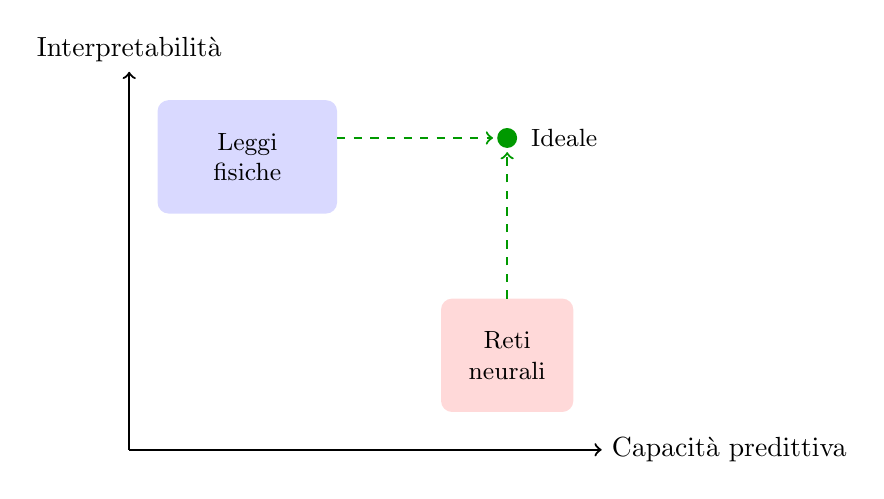
\begin{tikzpicture}[scale=1.2]
        % Assi
        \draw[->, thick] (0,0) -- (5,0) node[right] {Capacità predittiva};
        \draw[->, thick] (0,0) -- (0,4) node[above] {Interpretabilità};
        
        % Regione fisica classica
        \fill[blue!15, rounded corners] (0.3,2.5) rectangle (2.2,3.7);
        \node[align=center, font=\small] at (1.25,3.1) {Leggi\\fisiche};
        
        % Regione reti neurali
        \fill[red!15, rounded corners] (3.3,0.4) rectangle (4.7,1.6);
        \node[align=center, font=\small] at (4,1) {Reti\\neurali};
        
        % Punto ideale
        \fill[green!60!black] (4,3.3) circle (3pt);
        \node[anchor=west, font=\small] at (4.15,3.3) {Ideale};
        
        % Frecce tratteggiate verso l'ideale
        % Dalle reti neurali: dritta verso l'alto
        \draw[->, dashed, thick, green!60!black] (4,1.6) -- (4,3.15);
        % Dalle leggi fisiche: dritta verso destra
        \draw[->, dashed, thick, green!60!black] (2.2,3.3) -- (3.85,3.3);
        
    \end{tikzpicture}
    \caption{Il trade-off tra capacità predittiva e interpretabilità. Le leggi fisiche classiche sono interpretabili ma limitate nella complessità dei fenomeni che descrivono. Le reti neurali raggiungono capacità predittive elevate, ma producono rappresentazioni opache. L'obiettivo ideale è il punto di convergenza in alto a destra: modelli che uniscono la potenza predittiva alla trasparenza semantica.}
    \label{fig:tradeoff_prediction_interpretability}
\end{figure}
Questa asimmetria ha conseguenze profonde. Quando addestriamo una rete a fare previsioni, otteniamo una funzione—una mappa tra input e output che, in linea di principio, potrebbe contenere una legge. Ma a differenza delle leggi fisiche, di cui conosciamo il significato di ogni termine, nelle reti non sappiamo ricondurre i parametri a un significato. L'equazione $F = ma$ è potente non solo perché predice, ma perché ogni simbolo—forza, massa, accelerazione—ha un referente nel mondo. Una rete neurale con milioni di pesi può predire altrettanto bene, ma quei pesi non significano nulla per noi.
Ecco perché l'interpretabilità non è un lusso: è la condizione per estrarre conoscenza. Una rete che prevede ma non si lascia interpretare è uno strumento, non una teoria.
\subsubsection{La rete ideale}
Come sarebbe una rete neurale che unisce capacità predittiva e interpretabilità? Immaginiamo un modello in cui ogni neurone—ogni singola dimensione dello spazio delle attivazioni—corrisponda a esattamente un concetto semantico:
\begin{itemize}
    \item Il neurone 1 si attiva se e solo se l'input menziona un animale
    \item Il neurone 2 si attiva se e solo se la frase esprime sentimento negativo
    \item Il neurone 3 si attiva se e solo se il testo riguarda meccanica quantistica
    \item Il neurone 4 si attiva se e solo se si parla di torta al cioccolato
\end{itemize}
E così via, un neurone per ogni concetto che il modello deve rappresentare.
In un mondo così organizzato, interpretare il modello sarebbe immediato. Per sapere cosa la rete ha ``riconosciuto'' in un dato input, basterebbe osservare quali neuroni si sono attivati. Nessuna analisi sofisticata, nessuna tecnica di interpretabilità: la struttura stessa della rappresentazione renderebbe trasparente il funzionamento interno.
Modificare il comportamento del modello sarebbe altrettanto semplice. Se volessimo che la rete ignorasse il sentimento di una frase, basterebbe silenziare il neurone corrispondente. Se volessimo amplificare l'attenzione verso concetti culinari, basterebbe potenziare i neuroni dedicati a quel dominio. La rete parlerebbe la nostra lingua.
\subsubsection{Due spazi vettoriali}
Per formalizzare questa intuizione, dobbiamo distinguere due spazi vettoriali.
Il primo è lo spazio delle attivazioni. In una rete neurale, ogni layer produce un vettore di numeri reali—le attivazioni dei neuroni. Se il layer ha $n$ neuroni, le attivazioni formano un vettore in $\mathbb{R}^n$. Questo spazio ha una base naturale: gli assi corrispondono ai singoli neuroni. Scrivere $\mathbf{x} = (x_1, x_2, \dots, x_n)$ significa specificare l'attivazione di ciascun neurone.
\begin{notebox}
\textbf{Spazio delle attivazioni}\\
Lo spazio delle attivazioni è lo spazio vettoriale $\mathbb{R}^n$ in cui vivono gli output di un layer con $n$ neuroni. Ogni neurone definisce un asse di questo spazio. Lo stato della rete, in un dato istante e per un dato input, è un punto in questo spazio.
\end{notebox}
Il secondo è lo spazio delle feature. Questo è uno spazio concettuale: le sue dimensioni corrispondono ai concetti semantici che vorremmo rappresentare—``animale'', ``tristezza'', ``politica'', e così via. È lo spazio ideale in cui ogni direzione ha un significato che comprendiamo.
\begin{notebox}
\textbf{Spazio delle feature}\\
Lo spazio delle feature è lo spazio vettoriale $\mathbb{R}^m$ le cui dimensioni corrispondono a concetti semantici interpretabili. Se ci sono $m$ feature, un punto in questo spazio specifica l'intensità con cui ciascun concetto è presente. Questo spazio rappresenta l'immagine del mondo che la rete costruisce—e che vorremmo fosse allineata con la nostra.
\end{notebox}
La domanda centrale dell'interpretabilità diventa: qual è la relazione tra questi due spazi?
\subsubsection{Definizione di disentanglement}
Nel caso ideale, i due spazi coincidono perfettamente. Ogni neurone corrisponde a esattamente una feature, e ogni feature è catturata da esattamente un neurone. Questa configurazione è ciò che in letteratura viene chiamata rappresentazione disentangled~\parencite{wang2024disentangledrepresentationlearning}:
\begin{notebox}
\textbf{Rappresentazione Disentangled}\\
Una rappresentazione si dice \textit{disentangled} quando esiste una corrispondenza biunivoca tra lo spazio delle attivazioni e lo spazio delle feature:
\begin{enumerate}
    \item Ogni neurone (dimensione dello spazio delle attivazioni) codifica esattamente una feature
    \item Ogni feature (dimensione dello spazio semantico) è catturata da esattamente un neurone
\end{enumerate}
In termini formali, se $n$ è il numero di neuroni e $m$ il numero di feature, una rappresentazione perfettamente disentangled richiede $n = m$ e un isomorfismo tra i due spazi.
\end{notebox}
La Figura~\ref{fig:disentangled_vs_entangled} illustra la differenza tra una rappresentazione disentangled e una entangled.
\begin{figure}[htbp]
    \centering
    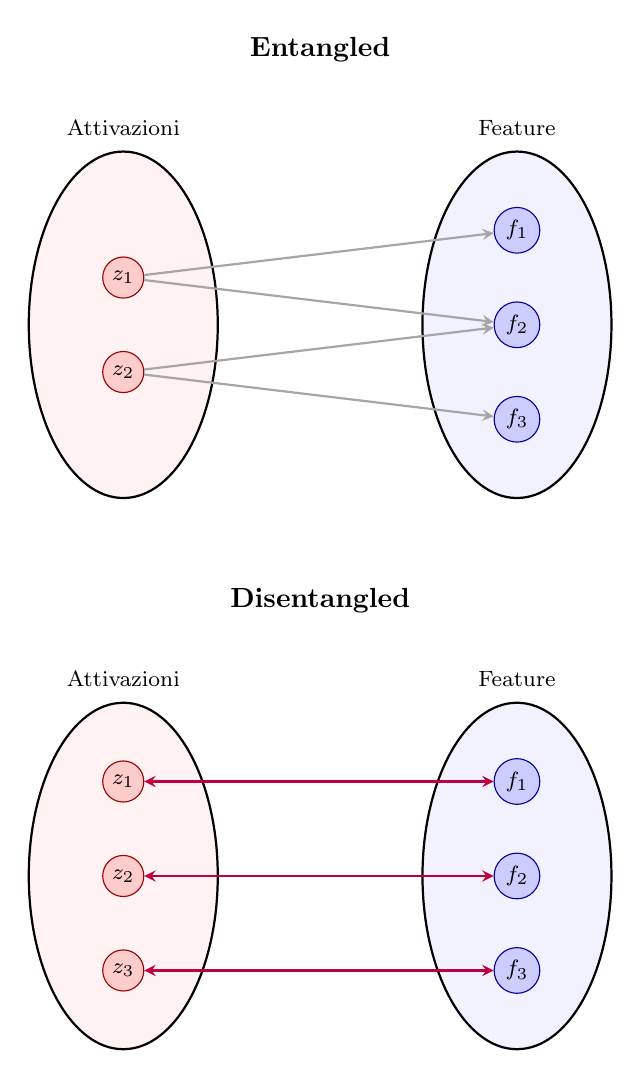
\begin{tikzpicture}
        
        % =========================================
        % === CASO ENTANGLED (In alto) ===
        % =========================================
        % Coordinate traslate orizzontalmente di -8 rispetto all'originale per centrarlo
        
        \node[font=\bfseries] at (2.5, 3.5) {Entangled};
        
        % Spazio delle attivazioni
        \draw[fill=red!5, thick] (0,0) ellipse (1.2cm and 2.2cm);
        \node[font=\footnotesize] at (0, 2.5) {Attivazioni};
        
        % Nodi Neuroni (meno neuroni che feature)
        \node[circle, fill=red!20, draw=red!60!black, inner sep=2pt, font=\footnotesize] (n1e) at (0, 0.6) {$z_1$};
        \node[circle, fill=red!20, draw=red!60!black, inner sep=2pt, font=\footnotesize] (n2e) at (0, -0.6) {$z_2$};

        % Spazio delle feature
        \draw[fill=blue!5, thick] (5,0) ellipse (1.2cm and 2.2cm);
        \node[font=\footnotesize] at (5, 2.5) {Feature};

        % Nodi Feature (più feature che neuroni)
        \node[circle, fill=blue!20, draw=blue!60!black, inner sep=2pt, font=\footnotesize] (c1e) at (5, 1.2) {$f_1$};
        \node[circle, fill=blue!20, draw=blue!60!black, inner sep=2pt, font=\footnotesize] (c2e) at (5, 0) {$f_2$};
        \node[circle, fill=blue!20, draw=blue!60!black, inner sep=2pt, font=\footnotesize] (c3e) at (5, -1.2) {$f_3$};

        % Frecce intrecciate (molti-a-molti)
        \draw[->, >=stealth, thick, gray!70] (n1e) -- (c1e);
        \draw[->, >=stealth, thick, gray!70] (n1e) -- (c2e);
        \draw[->, >=stealth, thick, gray!70] (n2e) -- (c2e);
        \draw[->, >=stealth, thick, gray!70] (n2e) -- (c3e);

        % =========================================
        % === CASO DISENTANGLED (In basso) ===
        % =========================================
        % Coordinate verticali (y) traslate di -7 rispetto all'originale per posizionarlo sotto
        
        \node[font=\bfseries] at (2.5, -3.5) {Disentangled};
        
        % Spazio delle attivazioni (centro y traslato a -7)
        \draw[fill=red!5, thick] (0,-7) ellipse (1.2cm and 2.2cm);
        \node[font=\footnotesize] at (0, -4.5) {Attivazioni};
        
        % Nodi Neuroni (y traslati di -7)
        \node[circle, fill=red!20, draw=red!60!black, inner sep=2pt, font=\footnotesize] (n1) at (0, -5.8) {$z_1$};
        \node[circle, fill=red!20, draw=red!60!black, inner sep=2pt, font=\footnotesize] (n2) at (0, -7) {$z_2$};
        \node[circle, fill=red!20, draw=red!60!black, inner sep=2pt, font=\footnotesize] (n3) at (0, -8.2) {$z_3$};

        % Spazio delle feature (centro y traslato a -7)
        \draw[fill=blue!5, thick] (5,-7) ellipse (1.2cm and 2.2cm);
        \node[font=\footnotesize] at (5, -4.5) {Feature};

        % Nodi Feature (y traslati di -7)
        \node[circle, fill=blue!20, draw=blue!60!black, inner sep=2pt, font=\footnotesize] (c1) at (5, -5.8) {$f_1$};
        \node[circle, fill=blue!20, draw=blue!60!black, inner sep=2pt, font=\footnotesize] (c2) at (5, -7) {$f_2$};
        \node[circle, fill=blue!20, draw=blue!60!black, inner sep=2pt, font=\footnotesize] (c3) at (5, -8.2) {$f_3$};

        % Frecce di corrispondenza biunivoca
        \draw[<->, >=stealth, thick, purple] (n1) -- (c1);
        \draw[<->, >=stealth, thick, purple] (n2) -- (c2);
        \draw[<->, >=stealth, thick, purple] (n3) -- (c3);
        
    \end{tikzpicture}
    \caption{Confronto tra rappresentazione entangled e disentangled. In alto: rappresentazione entangled con più feature che neuroni—ogni neurone partecipa alla codifica di più concetti, e ogni concetto è distribuito su più neuroni. In basso: rappresentazione disentangled con corrispondenza biunivoca tra neuroni e feature—ogni neurone codifica esattamente un concetto.}
    \label{fig:entangled_vs_disentangled_vert}
\end{figure}
Ma i modelli reali non funzionano così. E la ragione, come vedremo, non è una limitazione ingegneristica—è qualcosa di più profondo.
\subsection{Il paradosso della capacità}
\label{subsec:paradosso_capacita}
Se il mondo ideale richiede un neurone per ogni concetto, quanti neuroni servirebbero a un modello linguistico?
Consideriamo BERT-base, uno dei modelli più studiati. Ogni token viene rappresentato da un vettore di 768 dimensioni: 768 neuroni per ogni posizione nella sequenza, 768 numeri che devono catturare tutto ciò che il modello ``sa'' su quella parola in quel contesto.
Ma cosa ``sa'' BERT? L'elenco è impressionante. Il modello riconosce entità—persone, luoghi, organizzazioni, opere, prodotti—migliaia di categorie distinte. Comprende relazioni sintattiche: soggetto-verbo, modificatore-testa, dipendenze a lunga distanza. Cattura proprietà semantiche come animatezza, concretezza, polarità emotiva, registro linguistico. Possiede conoscenza enciclopedica: fatti storici, relazioni geografiche, proprietà degli oggetti. Distingue sfumature pragmatiche: ironia, understatement, formalità. È competente in domini specialistici: terminologia medica, legale, tecnica, scientifica.
Una stima conservativa suggerisce che un modello come BERT debba rappresentare decine di migliaia di concetti distinti per esibire le capacità che osserviamo empiricamente. Probabilmente molti di più.
Il problema ora è evidente:
\begin{equation}
    768 \text{ neuroni} \quad \ll \quad \text{decine di migliaia di concetti}
\end{equation}
Se ogni concetto richiedesse un neurone dedicato—come nella rappresentazione disentangled ideale—768 dimensioni permetterebbero al massimo 768 concetti. Ma BERT ne gestisce ordini di grandezza in più.
Eppure il modello funziona. Non solo funziona, ma raggiunge prestazioni straordinarie su una vasta gamma di compiti linguistici. Come è possibile?
La risposta a questo paradosso richiede di abbandonare un'assunzione implicita che abbiamo fatto finora—un'assunzione così naturale da sembrare ovvia, ma che si rivela essere il cuore del problema.
\subsection{Neuroni e feature: una distinzione cruciale}
\label{subsec:neuroni_feature}
L'assunzione nascosta è questa: abbiamo implicitamente identificato i neuroni con le feature. Abbiamo ragionato come se ogni concetto dovesse ``abitare'' in un neurone dedicato, e ogni neurone potesse ospitare un solo concetto. Ma queste due entità—neuroni e feature—sono oggetti profondamente diversi.
\begin{notebox}
\textbf{Neuroni vs Feature}
\begin{itemize}
    \item Un \textbf{neurone} (o dimensione) è un'unità computazionale della rete: un singolo valore numerico nello spazio delle attivazioni. I neuroni sono gli assi del sistema di coordinate—le direzioni ``cardinali'' lungo cui misuriamo le attivazioni. In BERT-base, ci sono 768 neuroni che definiscono gli assi $d_1, d_2, \dots, d_{768}$.    
    \item Una \textbf{feature} è un concetto semantico che il modello deve rappresentare: ``torta al cioccolato'', ``meccanica quantistica'', ``sentimento negativo''. Le feature sono le proprietà dei dati che risultano utili per i compiti del modello.
\end{itemize}
\end{notebox}
La chiave sta nel realizzare che le feature non devono necessariamente coincidere con gli assi. Una feature può essere rappresentata come una direzione arbitraria nello spazio—un vettore che punta in una direzione qualsiasi, combinando più neuroni con pesi diversi.
\subsubsection{L'analogia geografica}
Consideriamo un'analogia. Se dobbiamo descrivere la posizione di una città, possiamo usare le coordinate cardinali: ``100 km a Nord, 50 km a Est''. Gli assi Nord-Sud ed Est-Ovest sono i nostri ``neuroni''—le direzioni di riferimento del sistema. Ma nulla ci impedisce di descrivere la stessa posizione come ``112 km in direzione Nord-Nord-Est''. La direzione Nord-Nord-Est non coincide con nessun asse, ma è perfettamente definita come combinazione degli assi.
\begin{figure}[htbp]
    \centering
    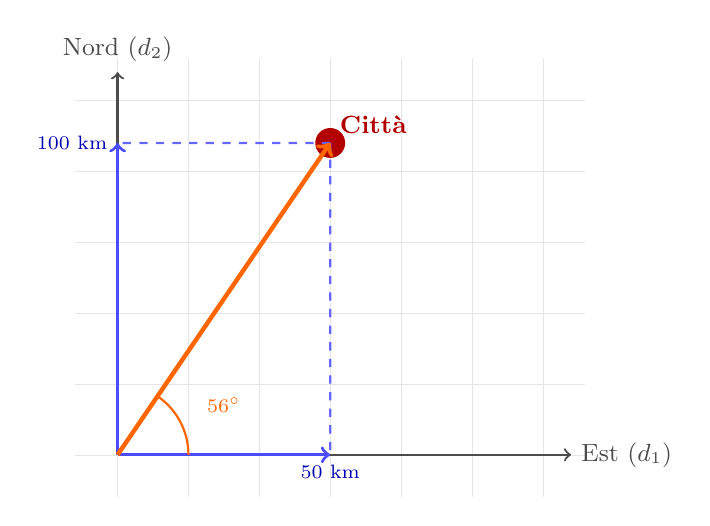
\begin{tikzpicture}[scale=1.8]
        % Griglia di sfondo
        \draw[gray!20, very thin, step=0.5] (-0.3,-0.3) grid (3.3,2.8);
        
        % Assi (neuroni)
        \draw[->, thick, black!70] (0,0) -- (3.2,0) node[right, font=\small] {Est ($d_1$)};
        \draw[->, thick, black!70] (0,0) -- (0,2.7) node[above, font=\small] {Nord ($d_2$)};
        
        % Punto di destinazione
        \coordinate (city) at (1.5, 2.2);
        \fill[red!70!black] (city) circle (3pt);
        \node[anchor=south west, font=\small\bfseries, red!70!black] at (city) {Città};
        
        % Componenti sugli assi (proiezioni tratteggiate)
        \draw[dashed, blue!60, thick] (city) -- (1.5, 0) node[below, font=\scriptsize, blue!70!black] {50 km};
        \draw[dashed, blue!60, thick] (city) -- (0, 2.2) node[left, font=\scriptsize, blue!70!black] {100 km};
        
        % Vettori componenti sugli assi
        \draw[->, very thick, blue!70] (0,0) -- (1.5, 0);
        \draw[->, very thick, blue!70] (0,0) -- (0, 2.2);
        
        % Direzione obliqua (la feature)
        \draw[->, ultra thick, orange!80!red] (0,0) -- (city);
        
        % Angolo
        \draw[orange!80!red, thick] (0.5,0) arc (0:56:0.5);
        % CORREZIONE QUI: Usato ^\circ invece di °
        \node[orange!80!red, font=\scriptsize] at (0.75, 0.35) {$56^\circ$};
        
    \end{tikzpicture} % Chiudo TikZ prima della caption
    
    % CORREZIONE QUI: Caption e Label spostate fuori da tikzpicture
    \caption{Analogia geografica tra neuroni e feature. Gli assi cardinali (Nord, Est) rappresentano i neuroni: le direzioni di riferimento del sistema. La direzione Nord-Nord-Est rappresenta una feature: non coincide con nessun asse, ma è definita come loro combinazione ($100 \text{ km Nord} + 50 \text{ km Est} = 112 \text{ km NNE}$). In uno spazio bidimensionale esistono solo 2 assi, ma infinite direzioni.}
    \label{fig:geographic_analogy}
\end{figure}
Allo stesso modo, una feature come ``torta al cioccolato'' non deve necessariamente corrispondere all'asse $d_{42}$. Può essere rappresentata come una direzione obliqua $\mathbf{w}_{\text{torta}}$ nello spazio delle attivazioni:
\begin{equation}
    \mathbf{w}_{\text{torta}} = 0.7 \cdot \mathbf{d}_1 + 0.5 \cdot \mathbf{d}_2 - 0.3 \cdot \mathbf{d}_3 + \dots
\end{equation}
una combinazione di molti neuroni, nessuno dei quali ``significa'' torta al cioccolato in isolamento.
\subsubsection{Direzioni e capacità}
Questa osservazione apre una possibilità che il ragionamento precedente escludeva: se le feature sono direzioni e non assi, possiamo avere più feature che neuroni. In uno spazio tridimensionale esistono solo tre assi, ma infinite direzioni.
\begin{notebox}
\textbf{Feature come direzioni}\\
Una feature è una direzione nello spazio vettoriale delle attivazioni. Indichiamo con $\mathbf{w}_i \in \mathbb{R}^{n}$ il vettore unitario associato alla feature $f_i$.
\end{notebox}
La domanda diventa: quante direzioni ``utili'' possiamo stipare in uno spazio a $n$ dimensioni? E a quale costo?
\subsection{La Superposition Hypothesis}
\label{subsec:superposition_hypothesis}
Se le feature sono direzioni, quante possiamo rappresentarne in uno spazio a $n$ dimensioni? La risposta dipende da un vincolo geometrico: quanto devono essere ``separate'' le direzioni per non confondersi tra loro.
\subsubsection{Il caso ideale: direzioni ortogonali}
Consideriamo uno spazio semplificato con soli due neuroni—due assi, $d_1$ e $d_2$—e supponiamo di avere esattamente due feature da rappresentare: $f_{\text{torta}}$ (``torta al cioccolato'') e $f_{\text{quant}}$ (``meccanica quantistica''). Con due neuroni a disposizione, possiamo assegnare a ciascuna feature un asse dedicato:
\begin{equation}
    \mathbf{w}_{\text{torta}} = \begin{pmatrix} 1 \\ 0 \end{pmatrix} = \mathbf{d}_1, \qquad
    \mathbf{w}_{\text{quant}} = \begin{pmatrix} 0 \\ 1 \end{pmatrix} = \mathbf{d}_2
\end{equation}
Questa è una rappresentazione perfettamente disentangled: ogni feature coincide con un asse. Le due direzioni sono ortogonali, il loro prodotto scalare è nullo ($\mathbf{w}_{\text{torta}} \cdot \mathbf{w}_{\text{quant}} = 0$), e questo significa che sono completamente indipendenti.
L'embedding $\mathbf{x}$ di un input si scrive come combinazione lineare:
\begin{equation}
    \mathbf{x} = a_{\text{torta}} \cdot \mathbf{w}_{\text{torta}} + a_{\text{quant}} \cdot \mathbf{w}_{\text{quant}} = \begin{pmatrix} a_{\text{torta}} \\ a_{\text{quant}} \end{pmatrix}
\end{equation}
dove $a_{\text{torta}}$ e $a_{\text{quant}}$ sono le intensità con cui ogni feature è presente nell'input.
Interpretare $\mathbf{x}$ è immediato: la prima coordinata indica direttamente l'intensità della feature $f_{\text{torta}}$, la seconda quella di $f_{\text{quant}}$. Nessuna ambiguità, nessuna interferenza.
\begin{figure}[htbp]
    \centering
    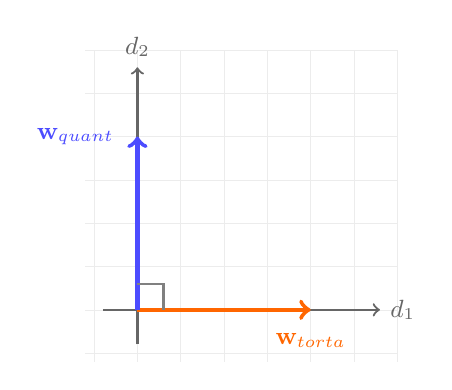
\begin{tikzpicture}[scale=2.2]
        % Griglia
        \draw[gray!15, very thin, step=0.25] (-0.3,-0.3) grid (1.5,1.5);        
        
        % Assi (neuroni)
        \draw[->, thick, black!60] (-0.2,0) -- (1.4,0) node[right, font=\small] {$d_1$};
        \draw[->, thick, black!60] (0,-0.2) -- (0,1.4) node[above, font=\small] {$d_2$};       
        
        % Feature allineate agli assi
        % Feature 1: Torta
        \draw[->, ultra thick, orange!80!red] (0,0) -- (1,0);
        \node[anchor=north, font=\small\bfseries, orange!80!red] at (1, -0.08) {$\mathbf{w}_{\text{torta}}$};        
        
        % Feature 2: Quantistica
        \draw[->, ultra thick, blue!70] (0,0) -- (0,1);
        \node[anchor=east, font=\small\bfseries, blue!70] at (-0.08, 1) {$\mathbf{w}_{\text{quant}}$};
        
        % Angolo retto (indicatore di ortogonalità)
        \draw[thick, black!50] (0.15,0) -- (0.15,0.15) -- (0,0.15);
        
    \end{tikzpicture}
    \caption{Rappresentazione disentangled ideale (2 feature, 2 neuroni). In questo scenario, le direzioni delle feature ($\mathbf{w}_i$) coincidono perfettamente con gli assi dei neuroni ($\mathbf{d}_i$). Questa configurazione garantisce \textbf{ortogonalità perfetta} ($\mathbf{w}_{\text{torta}} \cdot \mathbf{w}_{\text{quant}} = 0$): attivare il concetto di ``torta'' non crea alcuna interferenza sulla dimensione della ``meccanica quantistica''.}
    \label{fig:ideal_two_features}
\end{figure}
\subsubsection{Superposition: più feature che neuroni}
Aggiungiamo ora una terza feature: $f_{\text{ricetta}}$ (``ricetta di cucina''). Lo spazio ha solo due assi, ma tre feature da rappresentare. Nella logica disentangled, dovremmo rinunciare a una delle tre—non c'è spazio per tutte sugli assi.
Ma esiste un'alternativa. Se accettiamo che le direzioni $\mathbf{w}_i$ non debbano coincidere con gli assi, possiamo rappresentare tutte e tre le feature come direzioni nel piano. La configurazione geometricamente ottimale è quella che le distribuisce uniformemente: tre direzioni a 120° l'una dall'altra.
\begin{figure}[htbp]
    \centering
    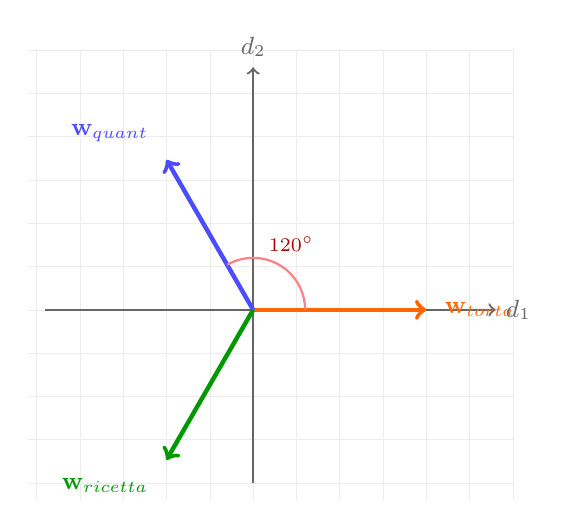
\begin{tikzpicture}[scale=2.2]
        % Griglia
        \draw[gray!15, very thin, step=0.25] (-1.3,-1.1) grid (1.5,1.5);
        
        % Assi (neuroni)
        \draw[->, thick, black!60] (-1.2,0) -- (1.4,0) node[right, font=\small] {$d_1$};
        \draw[->, thick, black!60] (0,-1.0) -- (0,1.4) node[above, font=\small] {$d_2$};
        
        % Tre feature a 120 gradi
        % Feature 1: Torta
        \draw[->, ultra thick, orange!80!red] (0,0) -- (1,0);
        \node[anchor=west, font=\small\bfseries, orange!80!red] at (1.05, 0) {$\mathbf{w}_{\text{torta}}$};
        
        % Feature 2: Quantistica
        \draw[->, ultra thick, blue!70] (0,0) -- ({cos(120)},{sin(120)});
        \node[anchor=south east, font=\small\bfseries, blue!70] at ({cos(120)-0.05},{sin(120)+0.05}) {$\mathbf{w}_{\text{quant}}$};
        
        % Feature 3: Ricetta
        \draw[->, ultra thick, green!60!black] (0,0) -- ({cos(240)},{sin(240)});
        \node[anchor=north east, font=\small\bfseries, green!60!black] at ({cos(240)-0.05},{sin(240)-0.05}) {$\mathbf{w}_{\text{ricetta}}$};
        
        % Indicatore Angolo
        \draw[red!50, thick] (0.3,0) arc (0:120:0.3);
        \node[red!70!black, font=\scriptsize] at (0.22, 0.38) {$120^\circ$};
        
    \end{tikzpicture}
    \caption{Il fenomeno della Superposition (3 feature in 2 dimensioni). A differenza del caso ideale, qui le direzioni delle feature ($\mathbf{w}_i$) non coincidono più con gli assi dei neuroni ($\mathbf{d}_i$). Per comprimere tre concetti in uno spazio bidimensionale mantenendo la massima distinguibilità possibile, i vettori si dispongono a $120^\circ$. Questa configurazione è un esempio di \textbf{quasi-ortogonalità}: il prodotto scalare non è zero, ma è minimizzato per ridurre le interferenze.}
    \label{fig:superposition_three_features}
\end{figure}
Questa configurazione è ciò che Elhage et al.~\parencite{elhage2022superposition} chiamano superposition: la rete rappresenta più feature di quanti siano i neuroni disponibili, codificando ogni feature come una direzione quasi-ortogonale nello spazio delle attivazioni.
\begin{notebox}
\textbf{Superposition Hypothesis}\\
Le reti neurali rappresentano $m$ feature in uno spazio di $n$ dimensioni, con $m > n$, codificando ogni feature $f_i$ come una direzione (vettore unitario) $\mathbf{w}_i$. Le direzioni sono scelte per essere il più possibile quasi-ortogonali—indipendenti nei limiti del vincolo dimensionale.
\end{notebox}
\subsubsection{Perché la superposition funziona: la sparsità}
La superposition sembra introdurre un problema: se le direzioni non sono ortogonali, come fa la rete a non confondere le feature? La risposta sta in un'osservazione empirica: le feature sono sparse.
Consideriamo i concetti che un modello linguistico deve rappresentare. ``Meccanica quantistica'' è rilevante solo in una minuscola frazione dei testi—articoli scientifici, manuali di fisica, discussioni specialistiche. ``Torta al cioccolato'' compare in contesti completamente diversi—ricette, blog culinari, menu di ristoranti. In un dato input, solo pochi concetti tra le migliaia possibili sono effettivamente pertinenti.
Questa sparsità rende la superposition vantaggiosa. Se due feature non sono mai attive contemporaneamente, possono condividere direzioni parzialmente sovrapposte senza mai interferire in pratica. La rete può ``stipare'' molte più feature di quanti siano i neuroni, accettando un piccolo rischio di interferenza nei rari casi di co-occorrenza.
\begin{figure}[htbp]
    \centering
    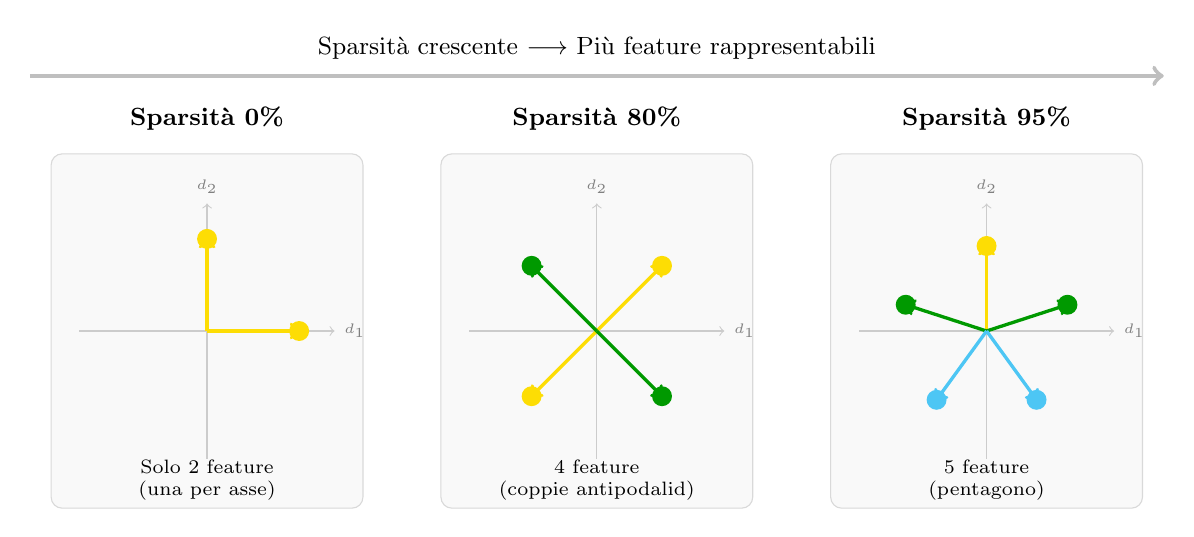
\begin{tikzpicture}[scale=0.9]    
        % === BOX 1: Sparsità 0% ===
        \draw[rounded corners, fill=gray!5, draw=gray!30] (-2.2,-2.5) rectangle (2.2,2.5);
        \node[font=\small\bfseries] at (0, 3) {Sparsità 0\%};     
        % Assi
        \draw[->, gray!40] (-1.8, 0) -- (1.8, 0) node[right, font=\tiny, gray] {$d_1$};
        \draw[->, gray!40] (0, -1.8) -- (0, 1.8) node[above, font=\tiny, gray] {$d_2$};
        % 2 feature sugli assi
        \draw[->, very thick, yellow!80!orange] (0,0) -- (1.3,0);
        \draw[->, very thick, yellow!80!orange] (0,0) -- (0,1.3);
        \fill[yellow!80!orange] (1.3,0) circle (4pt);
        \fill[yellow!80!orange] (0,1.3) circle (4pt);
        \node[font=\scriptsize, align=center, text width=2.5cm] at (0, -2.1) {
            Solo 2 feature\\(una per asse)
        };
        
        % === BOX 2: Sparsità 80% ===
        \begin{scope}[shift={(5.5,0)}]
            \draw[rounded corners, fill=gray!5, draw=gray!30] (-2.2,-2.5) rectangle (2.2,2.5);
            \node[font=\small\bfseries] at (0, 3) {Sparsità 80\%};
            % Assi
            \draw[->, gray!40] (-1.8, 0) -- (1.8, 0) node[right, font=\tiny, gray] {$d_1$};
            \draw[->, gray!40] (0, -1.8) -- (0, 1.8) node[above, font=\tiny, gray] {$d_2$};
            % 4 feature
            \draw[->, very thick, yellow!80!orange] (0,0) -- (0.92, 0.92);
            \draw[->, very thick, yellow!80!orange] (0,0) -- (-0.92, -0.92);
            \fill[yellow!80!orange] (0.92, 0.92) circle (4pt);
            \fill[yellow!80!orange] (-0.92, -0.92) circle (4pt);
            \draw[->, very thick, green!60!black] (0,0) -- (0.92, -0.92);
            \draw[->, very thick, green!60!black] (0,0) -- (-0.92, 0.92);
            \fill[green!60!black] (0.92, -0.92) circle (4pt);
            \fill[green!60!black] (-0.92, 0.92) circle (4pt);
            \node[font=\scriptsize, align=center, text width=2.8cm] at (0, -2.1) {
                4 feature\\(coppie antipodalid)
            };
        \end{scope}
        
        % === BOX 3: Sparsità 95% ===
        \begin{scope}[shift={(11,0)}]
            \draw[rounded corners, fill=gray!5, draw=gray!30] (-2.2,-2.5) rectangle (2.2,2.5);
            \node[font=\small\bfseries] at (0, 3) {Sparsità 95\%};
            % Assi
            \draw[->, gray!40] (-1.8, 0) -- (1.8, 0) node[right, font=\tiny, gray] {$d_1$};
            \draw[->, gray!40] (0, -1.8) -- (0, 1.8) node[above, font=\tiny, gray] {$d_2$};
            % 5 feature come pentagono
            \draw[->, very thick, yellow!80!orange] (0,0) -- ({1.2*cos(90)}, {1.2*sin(90)});
            \fill[yellow!80!orange] ({1.2*cos(90)}, {1.2*sin(90)}) circle (4pt);
            \draw[->, very thick, green!60!black] (0,0) -- ({1.2*cos(162)}, {1.2*sin(162)});
            \fill[green!60!black] ({1.2*cos(162)}, {1.2*sin(162)}) circle (4pt);
            \draw[->, very thick, green!60!black] (0,0) -- ({1.2*cos(18)}, {1.2*sin(18)});
            \fill[green!60!black] ({1.2*cos(18)}, {1.2*sin(18)}) circle (4pt);
            \draw[->, very thick, cyan!70] (0,0) -- ({1.2*cos(234)}, {1.2*sin(234)});
            \fill[cyan!70] ({1.2*cos(234)}, {1.2*sin(234)}) circle (4pt);
            \draw[->, very thick, cyan!70] (0,0) -- ({1.2*cos(306)}, {1.2*sin(306)});
            \fill[cyan!70] ({1.2*cos(306)}, {1.2*sin(306)}) circle (4pt);
            \node[font=\scriptsize, align=center, text width=2.8cm] at (0, -2.1) {
                5 feature\\(pentagono)
            };
        \end{scope}
        
        % Freccia sparsità crescente
        \draw[->, ultra thick, gray!50] (-2.5, 3.6) -- (13.5, 3.6);
        \node[font=\small, above] at (5.5, 3.7) {Sparsità crescente $\longrightarrow$ Più feature rappresentabili};
    \end{tikzpicture}
    \caption{Superposition al variare della sparsità (adattato da Elhage et al.~\parencite{elhage2022superposition}). Con sparsità crescente, la rete può rappresentare più feature nello stesso spazio, accettando direzioni sempre meno ortogonali.}
    \label{fig:sparsity_superposition}
\end{figure}
Questo spiega come BERT possa rappresentare decine di migliaia di concetti con soli 768 neuroni: le feature sono codificate come direzioni quasi-ortogonali, e la sparsità naturale del linguaggio garantisce che l'interferenza sia rara in pratica.
Ma la superposition ha un costo. Anche se funziona per la rete, crea due problemi fondamentali per chi vuole interpretarla.
\subsection{I due problemi della superposition}
\label{subsec:due_problemi}
La superposition permette alla rete di rappresentare molte più feature di quanti siano i neuroni disponibili. Ma questa compressione ha un costo: rende le rappresentazioni opache e difficili da decodificare.
Per capire perché, torniamo alla struttura matematica del problema. Nella superposition, l'embedding $\mathbf{x}$ di un input è una combinazione lineare delle direzioni delle feature:
\begin{equation}
    \mathbf{x} = \sum_i a_i \, \mathbf{w}_i
    \label{eq:linear_superposition}
\end{equation}
dove $\mathbf{w}_i$ è la direzione associata alla feature $f_i$ e $a_i$ è l'intensità con cui quella feature è presente nell'input.
Interpretare l'embedding significa rispondere a una domanda semplice: quali feature sono attive, e con quale intensità? In altre parole, dato $\mathbf{x}$, vogliamo recuperare le intensità $a_i$.
Questo problema ha due ostacoli fondamentali.
\subsubsection{Problema 1: l'opacità}
Il primo ostacolo è che non conosciamo le direzioni $\mathbf{w}_i$.
La rete ha appreso queste direzioni durante l'addestramento, ma non ce le rivela esplicitamente. Osserviamo solo il risultato finale—l'embedding $\mathbf{x}$—senza sapere quali direzioni lo compongono. È come ricevere un messaggio cifrato senza conoscere la chiave: l'informazione è presente, ma non sappiamo come estrarla.
Questo è il problema dell'opacità: l'informazione semantica è codificata in $\mathbf{x}$, ma non possiamo accedervi perché non conosciamo la ``mappa'' delle feature—le direzioni $\mathbf{w}_i$ che la rete usa internamente.
\subsubsection{Problema 2: l'interferenza}
Supponiamo, per un momento, di conoscere le direzioni $\mathbf{w}_i$. Potremmo allora recuperare le intensità $a_i$?
Nel caso ideale di direzioni ortogonali, la risposta sarebbe sì. Basterebbe calcolare il prodotto scalare tra $\mathbf{x}$ e la direzione $\mathbf{w}_i$:
\begin{equation}
    \mathbf{x} \cdot \mathbf{w}_i = a_i
\end{equation}
L'ortogonalità garantisce che ogni feature contribuisca solo alla propria componente, senza contaminare le altre.
Ma nella superposition le direzioni non sono ortogonali. Calcoliamo cosa succede quando proiettiamo $\mathbf{x}$ su una direzione $\mathbf{w}_i$:
\begin{equation}
    \mathbf{x} \cdot \mathbf{w}_i = \sum_j a_j \, (\mathbf{w}_j \cdot \mathbf{w}_i) = a_i + \sum_{j \neq i} a_j \, (\mathbf{w}_j \cdot \mathbf{w}_i)
    \label{eq:interference}
\end{equation}
Il primo termine è il segnale che cerchiamo: l'intensità $a_i$ della feature $f_i$. Il secondo termine è rumore: la somma dei contributi di tutte le altre feature, pesati per quanto le loro direzioni sono allineate con $\mathbf{w}_i$.
Solo se le direzioni fossero ortogonali ($\mathbf{w}_j \cdot \mathbf{w}_i = 0$ per $j \neq i$), il rumore svanirebbe. Nella superposition, questo non accade.
\subsubsection{Un esempio concreto}
Consideriamo l'esempio con tre feature a 120° (Figura~\ref{fig:superposition_three_features}). Le direzioni sono:
\begin{equation}
    \mathbf{w}_{\text{torta}} = \begin{pmatrix} 1 \\ 0 \end{pmatrix}, \quad
    \mathbf{w}_{\text{quant}} = \begin{pmatrix} -0.5 \\ 0.866 \end{pmatrix}, \quad
    \mathbf{w}_{\text{ricetta}} = \begin{pmatrix} -0.5 \\ -0.866 \end{pmatrix}
\end{equation}
Supponiamo che l'input riguardi solo torte al cioccolato: $a_{\text{torta}} = 1$, mentre $a_{\text{quant}} = a_{\text{ricetta}} = 0$. L'embedding è:
\begin{equation}
    \mathbf{x} = 1 \cdot \mathbf{w}_{\text{torta}} + 0 \cdot \mathbf{w}_{\text{quant}} + 0 \cdot \mathbf{w}_{\text{ricetta}} = \begin{pmatrix} 1 \\ 0 \end{pmatrix}
\end{equation}
Proviamo a decodificare quanto sembra attiva la feature ``meccanica quantistica'':
\begin{equation}
    \mathbf{x} \cdot \mathbf{w}_{\text{quant}} = \begin{pmatrix} 1 \\ 0 \end{pmatrix} \cdot \begin{pmatrix} -0.5 \\ 0.866 \end{pmatrix} = -0.5
\end{equation}
Il risultato è $-0.5$, non zero. Nonostante la feature ``meccanica quantistica'' sia completamente assente dall'input, la proiezione restituisce un valore non nullo. Questo è il rumore di interferenza: la non-ortogonalità delle direzioni causa attivazioni spurie.
\begin{figure}[htbp]
    \centering
    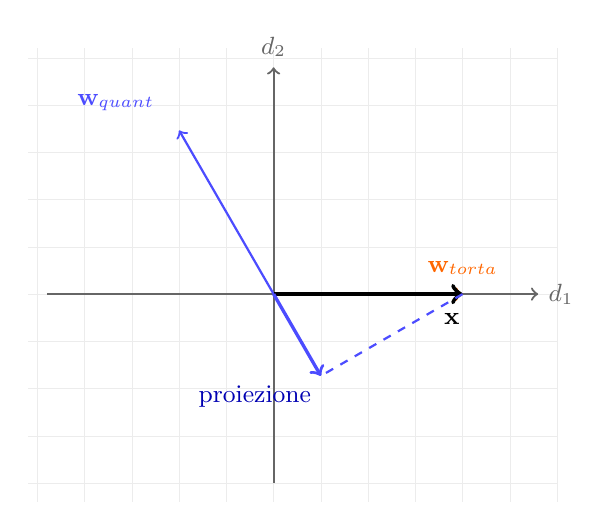
\begin{tikzpicture}[scale=2.4]
        % Griglia
        \draw[gray!15, very thin, step=0.25] (-1.3,-1.1) grid (1.5,1.3);
        
        % Assi (neuroni)
        \draw[->, thick, black!60] (-1.2,0) -- (1.4,0) node[right, font=\small] {$d_1$};
        \draw[->, thick, black!60] (0,-1.0) -- (0,1.2) node[above, font=\small] {$d_2$};
        
        % Direzioni delle feature
        % Torta
        \draw[->, thick, orange!80!red] (0,0) -- (1,0);
        \node[anchor=south, font=\small\bfseries, orange!80!red] at (1, 0.05) {$\mathbf{w}_{\text{torta}}$};
        
        % Quantistica
        \draw[->, thick, blue!70] (0,0) -- ({cos(120)},{sin(120)});
        \node[anchor=south east, font=\small\bfseries, blue!70] at ({cos(120)-0.08},{sin(120)+0.05}) {$\mathbf{w}_{\text{quant}}$};
        
        % Vettore x osservato (coincide con torta)
        \draw[->, ultra thick, black] (0,0) -- (1,0);
        \node[anchor=north west, font=\small] at (0.85, -0.05) {$\mathbf{x}$};
        
        % Proiezione di x su w_quant
        \coordinate (proj) at ({cos(120)*(-0.5)},{sin(120)*(-0.5)}); % Il coseno di 120 è -0.5, ma la proiezione è lungo la linea
        % Correzione geometrica per il disegno: la proiezione ortogonale cade a metà del vettore blu (ma con segno opposto se consideriamo il prodotto scalare)
        % Visivamente:
        \coordinate (p_point) at ({cos(120)}, 0); % No, proiezione di (1,0) sulla retta a 120°.
        % Proiezione scalare è 1 * cos(120) = -0.5. Quindi il punto è -0.5 * versore(120)
        \coordinate (proj_correct) at ({cos(120)*(-0.5)}, {sin(120)*(-0.5)}); 
        % Aspetta, -0.5 * versore vuol dire che va nella direzione opposta a w_quant (quindi a 300°/ -60°)
        % Ma per mostrare l'interferenza "sulla feature", solitamente si mostra la componente lungo l'asse della feature.
        % Disegnamolo geometricamente corretto: proiezione di (1,0) sulla retta definita da 120°.
        
        % Coordinate proiezione:
        \coordinate (projection) at ({cos(120)*cos(120)}, {cos(120)*sin(120)}); 
        
        \draw[dashed, blue!70, thick] (1,0) -- (projection);
        \draw[->, blue!70, very thick] (0,0) -- (projection);
        \node[blue!70!black, font=\small, anchor=north east] at (projection) {proiezione};
        
    \end{tikzpicture}
    \caption{Interferenza (\textit{Crosstalk}) nella Superposition. L'input contiene esclusivamente il concetto ``torta'' ($\mathbf{x} = \mathbf{w}_{\text{torta}}$), ma a causa della non-ortogonalità geometrica, si genera una proiezione non nulla sulla direzione ``quantistica''. Poiché $\mathbf{x} \cdot \mathbf{w}_{\text{quant}} = \cos(120^\circ) = -0.5$, il modello registra un'attivazione spuria (negativa) per un concetto assente. Questo ``rumore'' è il prezzo da pagare per rappresentare più feature che neuroni.}
    \label{fig:interference}
\end{figure}
\subsubsection{Riepilogo}
I due problemi della superposition si possono riassumere così:
\begin{notebox}
\textbf{I due problemi del disentanglement}\\[0.5em]
Vogliamo scrivere l'embedding come combinazione lineare di feature:
\begin{equation*}
    \mathbf{x} = \sum_i a_i \, \mathbf{w}_i
\end{equation*}
Ma:
\begin{enumerate}
    \item Non conosciamo le direzioni $\mathbf{w}_i$ (opacità)
    \item Non possiamo recuperare le intensità $a_i$ perché le direzioni non sono ortogonali (interferenza)
\end{enumerate}
\end{notebox}
Risolvere il problema del disentanglement significa affrontare entrambi questi ostacoli: trovare le direzioni delle feature e recuperare le intensità nonostante l'interferenza.

\subsection{L'idea del disentanglement}
\label{subsec:idea_disentanglement}

I due problemi della superposition—opacità e interferenza—sembrano intrattabili. Non conosciamo le direzioni $\mathbf{w}_i$, e anche se le conoscessimo non potremmo recuperare le intensità $a_i$ in modo pulito.

Ma la stessa proprietà che rende possibile la superposition—la sparsità delle feature—suggerisce una via d'uscita.

\subsubsection{Invertire la superposition}

Ricordiamo la situazione. In BERT, un embedding $\mathbf{x} \in \mathbb{R}^{768}$ codifica l'informazione relativa a molte feature $f_1, f_2, \dots, f_m$ simultaneamente:
\begin{equation}
    \mathbf{x} = \sum_{i=1}^{m} a_i \, \mathbf{w}_i
\end{equation}
dove $m \gg 768$. Le direzioni $\mathbf{w}_i$ sono sconosciute, le intensità $a_i$ sono sconosciute, e le direzioni non sono ortogonali. Questo è il problema.

L'obiettivo è costruire una rappresentazione dove l'informazione sia esplicita:
\begin{itemize}
    \item Ogni feature $f_i$ corrisponde a un asse dedicato—non a una direzione obliqua
    \item L'intensità $a_i$ è leggibile direttamente come coordinata lungo quell'asse
    \item Le feature sono separate—nessuna interferenza
\end{itemize}

In altre parole, vogliamo passare da uno spazio dove le feature sono direzioni sconosciute a uno spazio dove le feature sono assi noti. Vogliamo una rappresentazione $\mathbf{h}$ tale che:
\begin{equation}
    h_i \neq 0 \quad \Longleftrightarrow \quad \text{la feature } f_i \text{ è attiva nell'input}
\end{equation}

Questo è esattamente il mondo ideale disentangled che abbiamo descritto all'inizio del capitolo—ma con una differenza cruciale: non possiamo ottenerlo in 768 dimensioni, perché le feature sono molte di più.

\subsubsection{Lo spazio overcomplete}

La superposition esiste perché BERT deve rappresentare $m$ feature in $n < m$ dimensioni. Le feature vengono ``compresse'' come direzioni oblique perché non c'è abbastanza spazio per dare a ciascuna un asse dedicato.

Ma cosa succederebbe se avessimo abbastanza spazio? Se costruissimo un nuovo spazio con $q \geq m$ dimensioni—una per ogni feature—il problema della compressione svanirebbe. Ogni feature potrebbe avere il suo asse, e non ci sarebbe bisogno di superposition.

Questo è il punto di partenza: per invertire la superposition, dobbiamo espandere lo spazio, non comprimerlo.

Concretamente, definiamo un encoder—una funzione $f_\theta$—che mappa l'embedding originale in questo spazio espanso:
\begin{equation}
    \mathbf{h} = f_\theta(\mathbf{x}), \qquad \mathbf{h} \in \mathbb{R}^n, \quad n \gg d
\end{equation}

Questo spazio si dice overcomplete: ha più dimensioni dello spazio di partenza. Se BERT usa 768 dimensioni e le feature da rappresentare sono, diciamo, 50.000, allora scegliamo $n = 50.000$ o più. In questo spazio c'è abbastanza ``posto'' perché ogni feature abbia potenzialmente un asse dedicato.

\begin{figure}[htbp]
    \centering
    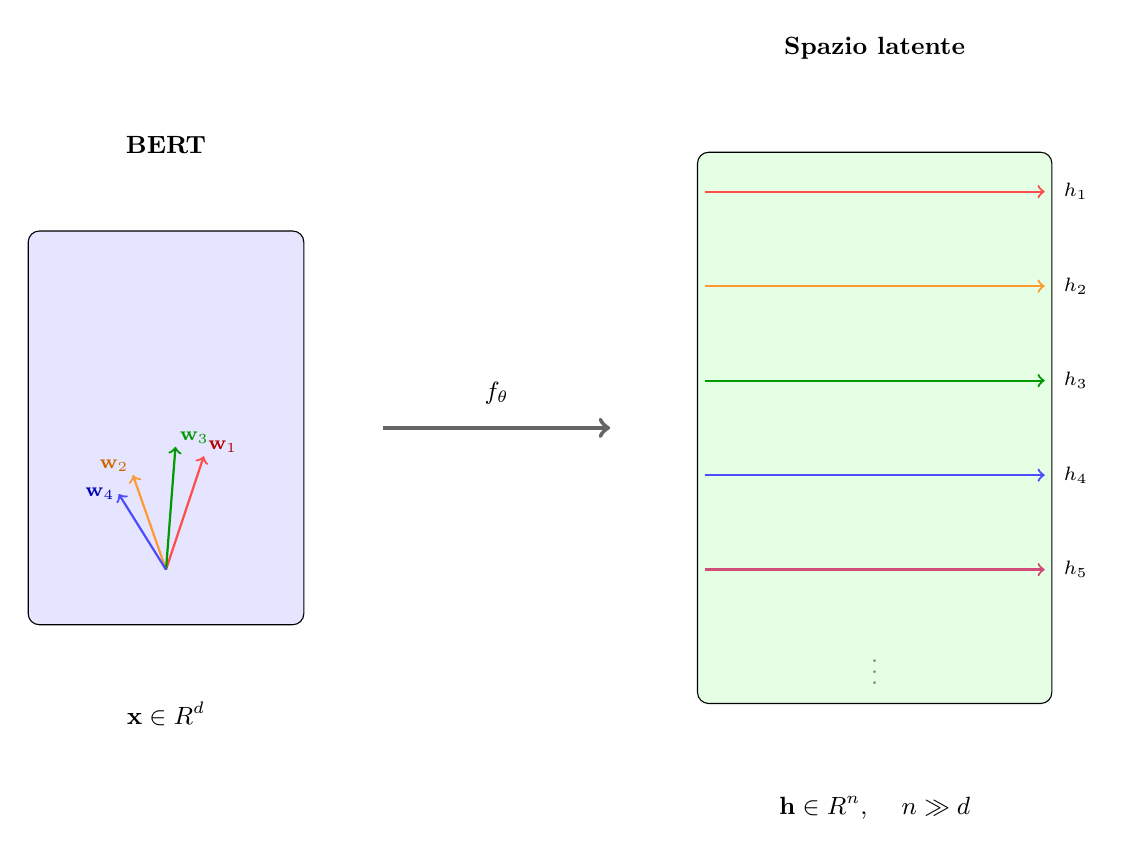
\begin{tikzpicture}[scale=1.2]
        % Spazio originale
        \node[draw, rectangle, minimum width=3.5cm, minimum height=5cm, fill=blue!10, rounded corners] (x) at (0,0) {};
        \node[above, font=\small\bfseries] at (0, 2.8) {BERT};
        
        % Frecce interne (direzioni oblique, mescolate)
        \coordinate (origin) at (0, -1.5);
        \draw[->, thick, red!70] (origin) -- ++(0.4, 1.2);
        \draw[->, thick, orange!80] (origin) -- ++(-0.35, 1.0);
        \draw[->, thick, green!60!black] (origin) -- ++(0.1, 1.3);
        \draw[->, thick, blue!70] (origin) -- ++(-0.5, 0.8);
        
        % Etichette
        \node[font=\scriptsize, red!70!black] at (0.6, -0.2) {$\mathbf{w}_1$};
        \node[font=\scriptsize, orange!80!black] at (-0.55, -0.4) {$\mathbf{w}_2$};
        \node[font=\scriptsize, green!60!black] at (0.3, -0.1) {$\mathbf{w}_3$};
        \node[font=\scriptsize, blue!70!black] at (-0.7, -0.7) {$\mathbf{w}_4$};
        
        \node[below, font=\small] at (0, -2.8) {$\mathbf{x} \in \mathbb{R}^{d}$};
        
        % Encoder
        \draw[->, ultra thick, black!60] (2.3, 0) -- (4.7, 0);
        \node[above, font=\small] at (3.5, 0.15) {$f_\theta$};
        
        % Spazio overcomplete
        \node[draw, rectangle, minimum width=4.5cm, minimum height=7cm, fill=green!10, rounded corners] (h) at (7.5,0) {};
        \node[above, font=\small\bfseries] at (7.5, 3.8) {Spazio latente};
        
        % Assi orizzontali (feature separate)
        \foreach \y/\c/\lab in {2.5/red!70/$h_1$, 1.5/orange!80/$h_2$, 0.5/green!60!black/$h_3$, -0.5/blue!70/$h_4$, -1.5/purple!70/$h_5$} {
            \draw[->, thick, \c] (5.7, \y) -- (9.3, \y);
            \node[font=\scriptsize, right] at (9.4, \y) {\lab};
        }
        
        \node[font=\small, gray] at (7.5, -2.5) {$\vdots$};
        
        \node[below, font=\small] at (7.5, -3.8) {$\mathbf{h} \in \mathbb{R}^{n}$, \quad $n \gg d$};
        
    \end{tikzpicture}
    \caption{Dall'embedding compresso allo spazio overcomplete. A sinistra, BERT codifica le feature come direzioni oblique $\mathbf{w}_i$ in $d$ dimensioni—mescolate e sconosciute (superposition). A destra, l'encoder $f_\theta$ proietta in uno spazio con $n \gg d$ dimensioni, dove ogni feature può avere un asse dedicato: la coordinata $h_i$ indica direttamente l'intensità della feature $f_i$.}
    \label{fig:overcomplete_space}
\end{figure}

\subsubsection{La sparsità come vincolo}

L'espansione dimensionale è necessaria, ma non sufficiente. Nulla garantisce, a priori, che l'encoder $f_\theta$ organizzi lo spazio $\mathbf{h}$ nel modo desiderato. Potremmo ritrovarci con 50.000 dimensioni in cui l'informazione è ancora mescolata e opaca—solo distribuita su più numeri.

Per ottenere una rappresentazione dove $h_i$ corrisponda effettivamente alla feature $f_i$, serve un vincolo che guidi l'apprendimento. Questo vincolo è la sparsità: per ogni input, solo poche coordinate di $\mathbf{h}$ possono essere attive.

L'intuizione è semplice. Se l'encoder può ``accendere'' solo un piccolo numero di dimensioni per rappresentare un input, ma deve comunque catturare tutta l'informazione necessaria alla ricostruzione, allora ogni dimensione è costretta a specializzarsi. Non può permettersi di codificare miscele ambigue di concetti—deve diventare un ``rilevatore'' dedicato a una specifica feature semantica.

È lo stesso principio che rende possibile la superposition, ma usato al contrario: là, la sparsità delle feature permetteva di comprimerle in poche dimensioni; qui, imponiamo sparsità alle attivazioni per forzare la separazione delle feature in dimensioni distinte.

\subsubsection{Il risultato: feature separate}

Quando l'addestramento converge, il risultato è una rappresentazione dove:
\begin{itemize}
    \item Ogni coordinata $h_i$ corrisponde a una feature $f_i$ specifica
    \item $h_i \neq 0$ indica che la feature è attiva nell'input
    \item Il valore di $h_i$ indica l'intensità della feature
\end{itemize}

Abbiamo invertito la superposition: le direzioni sconosciute $\mathbf{w}_i$ sono diventate assi noti $h_i$.

\begin{notebox}
\textbf{Disentanglement come proiezione}\\
Il disentanglement trasforma un embedding denso $\mathbf{x} \in \mathbb{R}^d$ in una rappresentazione sparsa $\mathbf{h} \in \mathbb{R}^n$ dove:
\begin{enumerate}
    \item $n > d$ (overcompletezza): abbastanza dimensioni per tutte le feature
    \item $\|\mathbf{h}\|_0 \ll n$ (sparsità): poche dimensioni attive per input
    \item $h_i$ indica l'intensità della feature $f_i$ (interpretabilità)
\end{enumerate}
In sintesi: spazio grande + attivazioni sparse = feature separate.
\end{notebox}

Resta una domanda: come apprendere questa mappa $f_\theta$? Come scoprire, dai dati, quali sono le feature e come proiettare gli embeddings nello spazio latente?
\subsection{Verso una soluzione: PRISMA}
\label{subsec:verso_soluzione}
La risposta viene da un'architettura neurale chiamata Sparse Autoencoder (SAE), che combina l'idea di ricostruzione tipica degli autoencoder con i vincoli di overcompletezza e sparsità che abbiamo discusso. I dettagli tecnici—l'architettura, la funzione di perdita, il processo di addestramento—saranno oggetto del prossimo capitolo.
Lì presenteremo PRISMA (\textbf{P}rojection of \textbf{R}epresentations for \textbf{I}nterpretability via \textbf{S}parse \textbf{M}onosemantic Autoencoders), un'applicazione sviluppata in questa tesi che implementa questo approccio. Il nome richiama un'analogia ottica: come un prisma scompone la luce bianca nelle sue componenti spettrali, così PRISMA scompone un embedding denso nelle sue feature semantiche costitutive.